% ============================================================
%  GUÍA DE REPASO — TEMA 1 (PRIMER LAPSO)
%  Números Naturales, Decimales, Potencias y Ecuaciones
%  Curso: 1er Año — CELAM
%  Autor: Ing. Gabriel Astudillo
%  Basada en las clases del 28/09/26 (memoria_clases.md)
% ============================================================

\documentclass[12pt, letterpaper]{article}

% ── Paquetes ─────────────────────────────────────────────────

\usepackage{mathwizards-guia}
\mwguia{Guía de Repaso — Tema 1}{Ing. Gabriel Astudillo $\cdot$ 1er Año}

% ── Comandos propios de esta guía ────────────────────────────
\newcommand{\N}{\mathbb{N}}
\newcommand{\Z}{\mathbb{Z}}

\begin{document}
% ============================================================

% ── Portada / Título ─────────────────────────────────────────
\mwportada{Guía de Repaso — Tema 1}{Naturales, Decimales, Potencias y Ecuaciones}{Todo el primer lapso en una sola guía}

\vspace{4pt}
\begin{cuadroinfo}
  \small
  \textbf{Presentación:} ¡Bienvenido a tu guía de repaso! Aquí reunimos \emph{todo} lo visto en el \textbf{Tema 1 del Primer Lapso}: los números naturales y su orden, las operaciones con decimales (suma, resta, multiplicación y división), la potenciación y radicación, las operaciones combinadas y las ecuaciones de primer grado en una incógnita. Cada sección empieza con la \textbf{teoría} resumida, sigue con \textbf{ejemplos resueltos} paso a paso y termina con \textbf{ejercicios progresivos} que van de lo más sencillo a los verdaderos retos. Al final encontrarás la \textbf{clave de respuestas} para comprobar tu trabajo.
  \\[4pt]
  \textbf{Nivel de Dificultad:}\quad
  \facil{} Básico / Directo \quad
  \medio{} Intermedio \quad
  \dificil{} Desafiante \quad
  \muyDificil{} Reto
\end{cuadroinfo}

\vspace{8pt}

% ============================================================
\section{Los Números Naturales y su Orden}
% ============================================================

\subsection{El conjunto de los números naturales}

Los números que usamos para \emph{contar} forman el conjunto de los \textbf{números naturales}.

\begin{cuadroteoria}
  \textbf{Definición:} el conjunto de los \textbf{números naturales} es
  \[
    \N = \{0,\ 1,\ 2,\ 3,\ 4,\ 5,\ \dots\}
  \]
  y \textbf{no tiene fin}: después de cada número siempre hay otro.
\end{cuadroteoria}

\noindent Podemos dibujarlos en la \textbf{recta numérica}, ordenados de menor a mayor hacia la derecha:

\begin{center}
  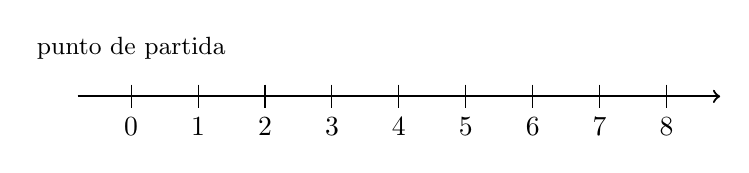
\begin{tikzpicture}[x=0.85cm]
    \draw[->, thick] (-0.8,0) -- (8.8,0);
    \foreach \x in {0,1,...,8} {
        \draw (\x,0.15) -- (\x,-0.15) node[below] {$\x$};
      }
    \node[above] at (0,0.35) {\small punto de partida};
  \end{tikzpicture}
\end{center}

\begin{cuadroteoria}
  \textbf{Relación de orden:} dados dos números naturales $a$ y $b$:
  \begin{itemize}[leftmargin=*]
    \item $a < b$ (se lee «$a$ es \textbf{menor que} $b$») si $a$ está a la izquierda de $b$.
    \item $a > b$ (se lee «$a$ es \textbf{mayor que} $b$») si $a$ está a la derecha de $b$.
    \item $a = b$ si representan la misma cantidad.
  \end{itemize}
  \textbf{Antecesor y sucesor:} el antecesor de $n$ es $n-1$ y el sucesor es $n+1$. Ejemplo: para $15$, el antecesor es $14$ y el sucesor es $16$.
\end{cuadroteoria}

\subsection{Ejercicios: Orden en $\N$}

\begin{enumerate}[leftmargin=*]
  \item \facil{} Coloca $<$, $>$ o $=$ según corresponda:
        \[ a)\; 7 \;\square\; 12 \qquad b)\; 25 \;\square\; 19 \qquad c)\; 100 \;\square\; 98 \qquad d)\; 40 \;\square\; 40 \]

  \item \facil{} Ordena de \textbf{menor a mayor}: $14,\ 3,\ 27,\ 9,\ 20$.

  \item \facil{} Ordena de \textbf{mayor a menor}: $45,\ 12,\ 38,\ 51,\ 7$.

  \item \medio{} Escribe el antecesor y el sucesor de: $a)\; 24 \qquad b)\; 99 \qquad c)\; 150$.

  \item \medio{} \textquestiondown Cuántos números naturales hay entre $17$ y $25$? (No los cuentes uno por uno; piensa en la diferencia.)

  \item \dificil{} Con las cifras $4$, $7$ y $1$ forma el \textbf{mayor} y el \textbf{menor} número de tres cifras posible, sin repetir cifras.

  \item \dificil{} Ordena de menor a mayor las siguientes estaturas en metros: $1{,}45;\ 1{,}5;\ 1{,}405;\ 1{,}54;\ 1{,}4$. (Compara con cuidado: las cifras decimales también se ordenan.)
\end{enumerate}

\newpage

% ============================================================
\section{Operaciones con Números Decimales}
% ============================================================

\subsection{Suma y resta de decimales}

Un \textbf{número decimal} usa una \textbf{coma} para separar la parte entera de la parte decimal: en $3{,}75$ la parte entera es $3$ y la parte decimal es $75$.

\begin{cuadropasos}
  \textbf{Pasos para sumar o restar decimales:}
  \begin{enumerate}
    \item \textbf{Alinea las comas} una debajo de la otra.
    \item \textbf{Completa con ceros} a la derecha si un número tiene menos cifras decimales.
    \item \textbf{Opera de derecha a izquierda} y coloca la coma en el mismo lugar.
  \end{enumerate}
  \textbf{Comprueba la resta:} si $a - b = c$, entonces $c + b = a$.
\end{cuadropasos}

\noindent\textbf{Ejemplo resuelto 1:} Calculemos $35{,}7 + 12{,}48$.

Completamos con un cero ($35{,}70$) y sumamos en columna:

\[
  \begin{array}{rr}
      & 35{,}70 \\
    + & 12{,}48 \\ \hline
      & 48{,}18
  \end{array}
\]

\noindent Respuesta: $35{,}7 + 12{,}48 = 48{,}18$.

\noindent\textbf{Ejemplo resuelto 2:} Calculemos $100 - 37{,}25$.

Completamos con ceros ($100{,}00$) y restamos:

\[
  \begin{array}{rr}
      & 100{,}00 \\
    - & 37{,}25   \\ \hline
      & 62{,}75
  \end{array}
\]

\noindent Comprobación: $62{,}75 + 37{,}25 = 100{,}00$. \textquestiondown Correcto! \checkmark

\begin{cuadroadvertencia}
  \textbf{Errores clásicos:} olvidar alinear las comas o no completar con ceros. Por ejemplo, $9{,}3 - 4{,}75$ \textbf{no} es $5{,}45$; el resultado correcto es $4{,}55$. \textquestiondown Siempre completa con ceros!
\end{cuadroadvertencia}

\subsection{Ejercicios: Suma y Resta}

\begin{enumerate}[leftmargin=*]
  \item \facil{} $12{,}5 + 3{,}4$

  \item \facil{} $8{,}75 + 4{,}5$

  \item \facil{} $0{,}6 + 0{,}9$

  \item \facil{} $25{,}4 - 13{,}2$

  \item \facil{} $9{,}3 - 4{,}75$

  \item \facil{} $100 - 36{,}5$

  \item \medio{} $145{,}75 + 89{,}6$

  \item \medio{} $2\,500 - 1\,347{,}85$

  \item \medio{} $34{,}085 + 230{,}4 + 1\,589{,}76$

  \item \medio{} Tenías $500$ Bs. y gastaste $348{,}65$ Bs. \textquestiondown Cuánto te queda?

  \item \medio{} $12{,}4 + 0{,}75 + 3{,}005$

  \item \dificil{} $145{,}125 + 234{,}875 + 1\,620{,}5$

  \item \dificil{} Sofía compra una licuadora de $48{,}25$ Bs., una cafetera de $136{,}60$ Bs. y un microondas de $257{,}15$ Bs. Si paga con un billete de $500$ Bs., \textquestiondown cuánto recibe de vuelto?

  \item \dificil{} $100 - 0{,}999$
\end{enumerate}

\vspace{6pt}

% ── Multiplicación ───────────────────────────────────────────
\subsection{Multiplicación de decimales}

Multiplicar es \emph{sumar varias veces lo mismo}. La clave está en saber dónde colocar la coma.

\begin{cuadropasos}
  \textbf{Pasos para multiplicar decimales:}
  \begin{enumerate}
    \item \textbf{Olvídate de la coma} y multiplica como si fueran números naturales.
    \item \textbf{Cuenta} el total de cifras decimales de los dos factores y \textbf{súmalas}.
    \item En el resultado, \textbf{cuenta esa misma cantidad de cifras de derecha a izquierda} y coloca ahí la coma.
  \end{enumerate}
\end{cuadropasos}

\noindent\textbf{Ejemplo resuelto 1:} Calculemos $2{,}5 \times 1{,}3$.

Multiplicamos sin coma: $25 \times 13 = 325$. Hay $1 + 1 = 2$ cifras decimales, entonces: $2{,}5 \times 1{,}3 = 3{,}25$.

\noindent\textbf{Ejemplo resuelto 2:} \textquestiondown Cuánto cuestan $4$ helados de $3{,}50$ Bs.?

\[
  4 \times 3{,}50 = 14{,}00 \quad\text{(la coma se conserva con dos cifras)}
\]

\noindent Los cuatro helados cuestan $14$ Bs.

\begin{cuadroadvertencia}
  \textbf{Potencia de $10$:} para multiplicar por $10$, $100$ o $1000$, solo \textbf{mueve la coma a la derecha} $1$, $2$ o $3$ lugares. Ejemplos: $4{,}25 \times 10 = 42{,}5$; \quad $0{,}7 \times 100 = 70$.
\end{cuadroadvertencia}

\subsection{Ejercicios: Multiplicación}

\begin{enumerate}[leftmargin=*]
  \item \facil{} $2{,}5 \times 3$

  \item \facil{} $0{,}4 \times 5$

  \item \facil{} $1{,}2 \times 4$

  \item \facil{} $3 \times 0{,}5$

  \item \medio{} $1\,250 \times 3{,}4$

  \item \medio{} $24{,}5 \times 1{,}2$

  \item \medio{} $650{,}8 \times 4{,}2$

  \item \medio{} $4\,500 \times 37{,}5$

  \item \medio{} En una tienda hay $240$ paquetes de galletas y cada uno cuesta $13{,}25$ Bs. \textquestiondown Cuánto cuestan todos juntos?

  \item \dificil{} $12{,}5 \times 0{,}08$

  \item \dificil{} $0{,}125 \times 4\,800$

  \item \dificil{} Un terreno rectangular mide $450{,}5$ m de largo y $230{,}4$ m de ancho. \textquestiondown Cuál es su área? (Área $=$ largo $\times$ ancho).

  \item \dificil{} \textquestiondown Cuánto cuestan $1\,200$ botellas de jugo si cada una cuesta $8{,}50$ Bs.?
\end{enumerate}

\newpage

% ── División ─────────────────────────────────────────────────
\subsection{División con decimales}

Dividir es \emph{repartir en partes iguales}. Cuando aparece una coma hay tres casos:

\begin{cuadroteoria}
  \textbf{Caso 1: Decimal entre entero.} Divide normalmente y, al bajar la coma del dividendo, coloca la coma en el cociente.
  \[
    4{,}8 \div 4 = 1{,}2
  \]

  \textbf{Caso 2: Entero entre decimal.} Multiplica \emph{los dos números} por $10$, $100$ o $1000$ para quitarle la coma al divisor y luego divide.
  \[
    3 \div 0{,}5 = 30 \div 5 = 6
  \]

  \textbf{Caso 3: Decimal entre decimal.} Igual que el caso 2: mueve la coma del divisor hasta que sea entero y mueve la del dividendo la misma cantidad de lugares.
  \[
    0{,}6 \div 0{,}12 = 60 \div 12 = 5
  \]
\end{cuadroteoria}

\begin{cuadropasos}
  \textbf{El método de la galera (paso a paso):}
  \begin{enumerate}
    \item Escribe el \textbf{dividendo} dentro de la galera y el \textbf{divisor} a la derecha.
    \item Pregúntate: \textquestiondown cuántas veces cabe el divisor en las primeras cifras?
    \item Escribe ese número en el \textbf{cociente}, \textbf{multiplica} y \textbf{resta}.
    \item \textbf{Baja} la siguiente cifra y repite hasta terminar.
    \item Si queda \textbf{resto}, coloca la coma en el cociente, agrega un \textbf{cero} al resto y continúa.
  \end{enumerate}
\end{cuadropasos}

\noindent\textbf{Ejemplo resuelto 1:} Calculemos $48{,}6 \div 3$.

\[
  \renewcommand{\arraystretch}{1.2}
  \begin{array}{r|l}
    48{,}6 & 3                   \\ \hline
           & \boldsymbol{16{,}2}
  \end{array}
  \qquad \text{Resto } = 0
\]

\noindent Comprobación: $16{,}2 \times 3 = 48{,}6$. \checkmark

\noindent\textbf{Ejemplo resuelto 2:} Calculemos $45 \div 0{,}5$.

Primero quitamos la coma del divisor multiplicando ambos números por $10$: $45 \div 0{,}5 = 450 \div 5 = 90$.

\noindent\textbf{Ejemplo resuelto 3:} Calculemos $7{,}56 \div 0{,}12$.

Multiplicamos ambos por $100$: $7{,}56 \div 0{,}12 = 756 \div 12 = 63$.

\begin{cuadroadvertencia}
  \textbf{Divisiones inexactas:} cuando el resto nunca llega a cero, la división es \textbf{inexacta}. En esta guía calcularemos el cociente \textbf{únicamente hasta dos cifras decimales (centésimas)}.
  \[
    14 \div 3 = 4{,}66 \quad \text{(resto } 0{,}02\text{)}
  \]
  \textbf{Comprobación:} $4{,}66 \times 3 + 0{,}02 = 13{,}98 + 0{,}02 = 14$. \checkmark
\end{cuadroadvertencia}

\subsection{Ejercicios: División}

\begin{enumerate}[leftmargin=*]
  \item \facil{} $84 \div 4$

  \item \facil{} $125 \div 5$

  \item \facil{} $2{,}4 \div 2$

  \item \facil{} $7{,}3 \div 3$ (dos cifras decimales)

  \item \medio{} $45 \div 0{,}5$

  \item \medio{} $0{,}6 \div 0{,}12$

  \item \medio{} $8{,}4 \div 0{,}7$

  \item \medio{} $156\,250 \div 25$

  \item \medio{} $486\,500 \div 12$ (dos cifras decimales)

  \item \dificil{} $15{,}625 \div 0{,}125$

  \item \dificil{} $3 \div 0{,}008$

  \item \dificil{} Tres hermanos se reparten en partes iguales un premio de $27{,}60$ Bs. \textquestiondown Cuánto recibe cada uno?

  \item \dificil{} Un rollo de tela de $25{,}5$ m se usa para confeccionar $7$ vestidos iguales. \textquestiondown Cuántos metros se emplean por vestido? (Dos cifras decimales.)

  \item \dificil{} $450 \div 0{,}7$ (dos cifras decimales)
\end{enumerate}

\newpage

% ============================================================
\section{Potenciación y Radicación en $\N$}
% ============================================================

\subsection{La potencia}

Multiplicar un número por sí mismo varias veces se escribe de forma corta con una \textbf{potencia}.

\begin{cuadroteoria}
  \textbf{Definición:} una \textbf{potencia} es una multiplicación repetida. Se escribe $a^n$ y se lee «$a$ elevado a la $n$».
  \[
    a^n = \underbrace{a \times a \times a \times \cdots \times a}_{n \text{ veces}}
  \]
  \begin{itemize}[leftmargin=*]
    \item \textbf{Base} ($a$): el número que se multiplica.
    \item \textbf{Exponente} ($n$): cuántas veces se multiplica.
    \item \textbf{Potencia}: el resultado.
  \end{itemize}
  Ejemplos: $2^3 = 8$, \quad $3^2 = 9$, \quad $10^3 = 1000$.
\end{cuadroteoria}

\begin{cuadroteoria}
  \textbf{Propiedades de las potencias (misma base):}
  \begin{itemize}[leftmargin=*]
    \item \textbf{Producto:} $a^m \times a^n = a^{m+n}$. Ejemplo: $2^3 \times 2^2 = 2^5 = 32$.
    \item \textbf{Cociente:} $a^m \div a^n = a^{m-n}$. Ejemplo: $5^4 \div 5^2 = 5^2 = 25$.
    \item \textbf{Potencia de potencia:} $(a^m)^n = a^{m\times n}$. Ejemplo: $(3^2)^3 = 3^6 = 729$.
    \item Todo número elevado a $1$ es él mismo: $a^1 = a$. \quad Todo número (distinto de $0$) elevado a $0$ es $1$: $a^0 = 1$.
  \end{itemize}
\end{cuadroteoria}

\subsection{La radicación}

La \textbf{raíz} es la operación \emph{inversa} de la potencia.

\begin{cuadroteoria}
  \[
    \sqrt[n]{a} = b \quad \Longleftrightarrow \quad b^n = a
  \]
  \begin{itemize}[leftmargin=*]
    \item \textbf{Raíz cuadrada} ($n = 2$): $\sqrt{49} = 7$ porque $7^2 = 49$.
    \item \textbf{Raíz cúbica} ($n = 3$): $\sqrt[3]{8} = 2$ porque $2^3 = 8$.
  \end{itemize}
\end{cuadroteoria}

\noindent\textbf{Ejemplo resuelto:} Calculemos $2^5 \times 3^2$.

$$2^5 = 32 \qquad 3^2 = 9 \qquad 32 \times 9 = 288$$

\subsection{Ejercicios: Potencias y Raíces}

\begin{enumerate}[leftmargin=*]
  \item \facil{} $3^2$

  \item \facil{} $2^5$

  \item \facil{} $5^3$

  \item \facil{} $10^4$

  \item \facil{} $\sqrt{16}$

  \item \facil{} $\sqrt{49}$

  \item \medio{} $\sqrt[3]{8}$

  \item \medio{} $4^3$

  \item \medio{} $6^2$

  \item \medio{} $2^3 \times 2^2$

  \item \medio{} $5^4 \div 5^2$

  \item \medio{} $(3^2)^3$

  \item \dificil{} $2^5 \times 3^2$

  \item \dificil{} $\sqrt{25 \times 4}$

  \item \dificil{} $(2^3)^2 \div 4^2$

  \item \dificil{} Un tablero de ajedrez tiene $8 \times 8$ casillas. \textquestiondown Cuántas casillas hay? Exprésalo como potencia y calcúlalo.

  \item \dificil{} \textquestiondown Cuál es el número cuyo cuadrado es $144$?
\end{enumerate}

\newpage

% ============================================================
\section{Operaciones Combinadas en $\N$}
% ============================================================

\subsection{El orden de las operaciones}

En una expresión con varias operaciones \textbf{no} se resuelve de izquierda a derecha: hay una \textbf{jerarquía} que debemos respetar.

\begin{cuadroteoria}
  \textbf{Orden para resolver operaciones combinadas:}
  \begin{enumerate}[leftmargin=*]
    \item \textbf{Signos de agrupación}, de adentro hacia afuera: paréntesis $(\ )$, corchetes $[\ ]$, llaves $\{\ \}$.
    \item \textbf{Potencias y raíces}.
    \item \textbf{Multiplicaciones y divisiones}, de izquierda a derecha.
    \item \textbf{Sumas y restas}, de izquierda a derecha.
  \end{enumerate}
\end{cuadroteoria}

\noindent\textbf{Ejemplo resuelto 1:} Calculemos $5 + 2 \times (3^2 - 4)$.

Resolvemos el paréntesis (dentro, primero la potencia): $3^2 - 4 = 9 - 4 = 5$. Luego la multiplicación: $2 \times 5 = 10$. Finalmente la suma: $5 + 10 = 15$.

\noindent\textbf{Ejemplo resuelto 2:} Calculemos $20 - [\,3 \times (2 + 4) - \sqrt{16}\,]$.

Paréntesis: $2 + 4 = 6$. Corchete: $3 \times 6 - 4 = 18 - 4 = 14$. Resultado: $20 - 14 = 6$.

\begin{cuadroadvertencia}
  \textbf{¡Ojo con el orden!} $2 + 3 \times 4 = 2 + 12 = 14$, pero $(2 + 3) \times 4 = 5 \times 4 = 20$. Un paréntesis cambia todo el resultado: respeta siempre la jerarquía.
\end{cuadroadvertencia}

\subsection{Ejercicios: Operaciones Combinadas}

\begin{enumerate}[leftmargin=*]
  \item \facil{} $5 + 3 \times 2$

  \item \facil{} $(5 + 3) \times 2$

  \item \facil{} $12 - 4 \div 2$

  \item \facil{} $2^2 + 5$

  \item \facil{} $10 - \sqrt{9}$

  \item \medio{} $4 + 2 \times (8 - 3)$

  \item \medio{} $3^2 + 4 \times 2 - 5$

  \item \medio{} $20 \div (2 + 3) + 6$

  \item \medio{} $\sqrt{36} + 2^3 - 5$

  \item \medio{} $(7 + 5) \times (9 - 6)$

  \item \dificil{} $15 - [\,2 \times (7 - 4) + 3\,]$

  \item \dificil{} $4 \times \{\,2 + 3 \times [\,10 - 2 \times (4 - 2)\,]\,\}$

  \item \dificil{} $2^3 + \sqrt{25} \times (6 - 4) - 10 \div 2$

  \item \dificil{} $[\,3^2 - (2 + 5)\,] \times \sqrt{4} + 6$

  \item \dificil{} En una tienda hay $5$ cajas con $12$ lápices cada una. Se venden $3$ cajas y luego llegan $2$ cajas más con $10$ lápices cada una. \textquestiondown Cuántos lápices hay ahora? Escríbelo en \textbf{una sola expresión} y calcula.
\end{enumerate}

% ============================================================
\section{Ecuaciones de Primer Grado en una Incógnita}
% ============================================================

\subsection{La ecuación y sus partes}

Una \textbf{ecuación} es una igualdad donde una letra (la \textbf{incógnita}) esconde un número que queremos descubrir. Es como una \textbf{balanza} en equilibrio.

\begin{cuadroteoria}
  \[
    \underbrace{2x + 3}_{\text{1er miembro}} = \underbrace{11}_{\text{2do miembro}}
  \]
  \begin{itemize}[leftmargin=*]
    \item \textbf{Miembros:} cada lado de la igualdad.
    \item \textbf{Incógnita:} la letra desconocida ($x$).
    \item \textbf{Términos:} cada parte que se suma o se resta ($2x$ y $3$).
    \item \textbf{Coeficiente:} el número que multiplica a la incógnita (el $2$ de $2x$).
  \end{itemize}
\end{cuadroteoria}

\noindent\textbf{Regla de oro:} todo lo que hagas en un miembro, \textbf{hazlo también en el otro}. Así la balanza nunca se desequilibra. Para «deshacer» lo que le pasa a la incógnita usamos la \textbf{operación inversa}: la suma se deshace con la resta, y la multiplicación con la división.

\begin{cuadropasos}
  \textbf{Pasos para resolver una ecuación:}
  \begin{enumerate}
    \item \textbf{Elimina} los signos de agrupación (aplica la propiedad distributiva: $a(b + c) = ab + ac$).
    \item \textbf{Agrupa} los términos semejantes (las $x$ con las $x$, los números con los números).
    \item \textbf{Transpone:} pasa los términos de un lado cambiando su signo (+ pasa a $-$ y $-$ pasa a $+$).
    \item \textbf{Despeja} la incógnita (si queda $ax = b$, entonces $x = b \div a$).
    \item \textbf{Comprueba} sustituyendo el valor en la ecuación original.
  \end{enumerate}
\end{cuadropasos}

\noindent\textbf{Ejemplo resuelto 1:} Resuelve $x + 8 = 15$.

Restamos $8$ en ambos lados: $x = 15 - 8 = 7$. \quad Comprobación: $7 + 8 = 15$. \checkmark

\noindent\textbf{Ejemplo resuelto 2:} Resuelve $3(x + 2) = 18$.

Aplicamos distributiva: $3x + 6 = 18 \;\Rightarrow\; 3x = 12 \;\Rightarrow\; x = 4$. \quad Comprobación: $3(4 + 2) = 3 \times 6 = 18$. \checkmark

\noindent\textbf{Ejemplo resuelto 3 (con muchos términos):} Resuelve $5x + 3 - 2x = 15 - x$.

Agrupamos: $3x + 3 = 15 - x$. Transponemos: $3x + x = 15 - 3 \;\Rightarrow\; 4x = 12 \;\Rightarrow\; x = 3$. \quad Comprobación: $5(3) + 3 - 2(3) = 15 + 3 - 6 = 12$ y $15 - 3 = 12$. \checkmark

\begin{cuadroadvertencia}
  \textbf{\textquestiondown La solución no pertenece a $\N$?} Como trabajamos en los naturales, a veces la solución es negativa (o no entera), y eso significa que \textbf{no pertenece a $\N$}. En esos casos \textbf{no se comprueba} y se escribe:
  \[
    x + 3 = 1 \;\Rightarrow\; x = -2 \quad\text{y colocamos}\quad x \notin \N
  \]
\end{cuadroadvertencia}

\subsection{Ejercicios: Ecuaciones}

\begin{enumerate}[leftmargin=*]
  \item \facil{} $x + 6 = 14$

  \item \facil{} $x - 5 = 9$

  \item \facil{} $4x = 24$

  \item \facil{} $\dfrac{x}{3} = 5$

  \item \facil{} $2x + 3 = 13$

  \item \facil{} $5x - 4 = 21$

  \item \medio{} $3x + 7 = 2x + 15$

  \item \medio{} $5x - 3 = 3x + 9$

  \item \medio{} $2(x + 4) = 20$

  \item \medio{} $3(x - 2) = x + 8$

  \item \medio{} $4x + 2 - 2x = 3x - 5$

  \item \medio{} $x + 3 = 1$ (recuerda la nota: si no pertenece a $\N$, escribe $x \notin \N$)

  \item \dificil{} $5(x - 1) = 3x + 7$

  \item \dificil{} $6x - 2(3 - x) = 3(x + 2) + 8$

  \item \dificil{} $8x - 3 + 2x = 5x + 12 + 10$

  \item \dificil{} $3x + 5 = 2x + 1$

  \item \medio{} El doble de un número aumentado en $7$ es igual a $25$. \textquestiondown Cuál es el número?

  \item \dificil{} La suma de tres números consecutivos es $48$. \textquestiondown Cuál es el menor de ellos?

  \item \dificil{} Pienso un número, le sumo $9$ y obtengo $4$. \textquestiondown Cuál es el número? \textquestiondown Pertenece a $\N$?
\end{enumerate}

\newpage

% ============================================================
\ifmwclaves
  \section{Clave de Respuestas}
  % ============================================================

  \subsection*{Orden en $\N$}
  \begin{enumerate}[leftmargin=*, label=\textbf{\arabic*.}]
    \item $a)\; 7 < 12$; \quad $b)\; 25 > 19$; \quad $c)\; 100 > 98$; \quad $d)\; 40 = 40$.
    \item $3,\ 9,\ 14,\ 20,\ 27$.
    \item $51,\ 45,\ 38,\ 12,\ 7$.
    \item $a)$ antecesor $23$, sucesor $25$; \quad $b)$ $98$ y $100$; \quad $c)$ $149$ y $151$.
    \item Hay $7$ números ($18, 19, 20, 21, 22, 23, 24$).
    \item Mayor: $741$; \quad menor: $147$.
    \item $1{,}4;\ 1{,}405;\ 1{,}45;\ 1{,}5;\ 1{,}54$.
  \end{enumerate}

  \subsection*{Suma y Resta}
  \begin{enumerate}[leftmargin=*, label=\textbf{\arabic*.}]
    \item $15{,}9$
    \item $13{,}25$
    \item $1{,}5$
    \item $12{,}2$
    \item $4{,}55$
    \item $63{,}5$
    \item $145{,}75 + 89{,}6 = 235{,}35$
    \item $2\,500 - 1\,347{,}85 = 1\,152{,}15$
    \item $34{,}085 + 230{,}4 + 1\,589{,}76 = 1\,854{,}245$
    \item $500 - 348{,}65 = 151{,}35$ Bs.
    \item $12{,}4 + 0{,}75 + 3{,}005 = 16{,}155$
    \item $145{,}125 + 234{,}875 + 1\,620{,}5 = 2\,000{,}5$
    \item Total: $48{,}25 + 136{,}60 + 257{,}15 = 442{,}00$ Bs. Vuelto: $500 - 442 = 58$ Bs.
    \item $100 - 0{,}999 = 99{,}001$
  \end{enumerate}

  \subsection*{Multiplicación}
  \begin{enumerate}[leftmargin=*, label=\textbf{\arabic*.}]
    \item $7{,}5$
    \item $2$
    \item $4{,}8$
    \item $1{,}5$
    \item $1\,250 \times 3{,}4 = 4\,250$
    \item $24{,}5 \times 1{,}2 = 29{,}4$
    \item $650{,}8 \times 4{,}2 = 2\,733{,}36$
    \item $4\,500 \times 37{,}5 = 168\,750$
    \item $240 \times 13{,}25 = 3\,180$ Bs.
    \item $12{,}5 \times 0{,}08 = 1$
    \item $0{,}125 \times 4\,800 = 600$
    \item $450{,}5 \times 230{,}4 = 103\,795{,}2$ m$^2$
    \item $1\,200 \times 8{,}50 = 10\,200$ Bs.
  \end{enumerate}

  \subsection*{División}
  \begin{enumerate}[leftmargin=*, label=\textbf{\arabic*.}]
    \item $21$
    \item $25$
    \item $1{,}2$
    \item $7{,}3 \div 3 = 2{,}43$ (resto $0{,}01$)
    \item $45 \div 0{,}5 = 450 \div 5 = 90$
    \item $0{,}6 \div 0{,}12 = 60 \div 12 = 5$
    \item $8{,}4 \div 0{,}7 = 84 \div 7 = 12$
    \item $156\,250 \div 25 = 6\,250$
    \item $486\,500 \div 12 = 40\,541{,}66$ (resto $0{,}08$)
    \item $15{,}625 \div 0{,}125 = 125$
    \item $3 \div 0{,}008 = 3000 \div 8 = 375$
    \item $27{,}60 \div 3 = 9{,}20$ Bs.
    \item $25{,}5 \div 7 = 3{,}64$ m (resto $0{,}02$ m)
    \item $450 \div 0{,}7 = 4\,500 \div 7 = 642{,}85$ (resto $0{,}05$)
  \end{enumerate}

  \subsection*{Potencias y Raíces}
  \begin{enumerate}[leftmargin=*, label=\textbf{\arabic*.}]
    \item $9$
    \item $32$
    \item $125$
    \item $10\,000$
    \item $4$
    \item $7$
    \item $2$
    \item $64$
    \item $36$
    \item $2^3 \times 2^2 = 2^5 = 32$
    \item $5^4 \div 5^2 = 5^2 = 25$
    \item $(3^2)^3 = 3^6 = 729$
    \item $2^5 \times 3^2 = 32 \times 9 = 288$
    \item $\sqrt{25 \times 4} = \sqrt{100} = 10$
    \item $(2^3)^2 \div 4^2 = 64 \div 16 = 4$
    \item $8^2 = 64$ casillas.
    \item $12$, porque $12^2 = 144$.
  \end{enumerate}

  \subsection*{Operaciones Combinadas}
  \begin{enumerate}[leftmargin=*, label=\textbf{\arabic*.}]
    \item $5 + 6 = 11$
    \item $8 \times 2 = 16$
    \item $12 - 2 = 10$
    \item $4 + 5 = 9$
    \item $10 - 3 = 7$
    \item $4 + 2 \times 5 = 4 + 10 = 14$
    \item $9 + 8 - 5 = 12$
    \item $20 \div 5 + 6 = 4 + 6 = 10$
    \item $6 + 8 - 5 = 9$
    \item $12 \times 3 = 36$
    \item $15 - [\,2 \times 3 + 3\,] = 15 - 9 = 6$
    \item $4 \times \{\,2 + 3 \times 6\,\} = 4 \times 20 = 80$
    \item $8 + 5 \times 2 - 5 = 8 + 10 - 5 = 13$
    \item $[\,9 - 7\,] \times 2 + 6 = 4 + 6 = 10$
    \item $(5 - 3) \times 12 + 2 \times 10 = 24 + 20 = 44$ lápices.
  \end{enumerate}

  \subsection*{Ecuaciones}
  \begin{enumerate}[leftmargin=*, label=\textbf{\arabic*.}]
    \item $x = 8$
    \item $x = 14$
    \item $x = 6$
    \item $x = 15$
    \item $2x = 10 \Rightarrow x = 5$
    \item $5x = 25 \Rightarrow x = 5$
    \item $3x - 2x = 15 - 7 \Rightarrow x = 8$
    \item $5x - 3x = 9 + 3 \Rightarrow 2x = 12 \Rightarrow x = 6$
    \item $2x + 8 = 20 \Rightarrow 2x = 12 \Rightarrow x = 6$
    \item $3x - 6 = x + 8 \Rightarrow 2x = 14 \Rightarrow x = 7$
    \item $2x + 2 = 3x - 5 \Rightarrow x = 7$
    \item $x = 1 - 3 = -2$; como $-2$ es negativo, $x \notin \N$.
    \item $5x - 5 = 3x + 7 \Rightarrow 2x = 12 \Rightarrow x = 6$
    \item $8x - 6 = 3x + 14 \Rightarrow 5x = 20 \Rightarrow x = 4$
    \item $10x - 3 = 5x + 22 \Rightarrow 5x = 25 \Rightarrow x = 5$
    \item $x = 1 - 5 = -4$; como $-4$ es negativo, $x \notin \N$.
    \item $2x + 7 = 25 \Rightarrow 2x = 18 \Rightarrow x = 9$.
    \item $n + (n+1) + (n+2) = 48 \Rightarrow 3n + 3 = 48 \Rightarrow n = 15$. El menor es $15$.
    \item $x + 9 = 4 \Rightarrow x = -5$; como $-5$ es negativo, $x \notin \N$.
  \end{enumerate}

  \vspace{10pt}
  \begin{cuadrosolucion}
    \textbf{\textquestiondown Cómo te fue?} Si resolviste hasta el final, ya dominas todo el Tema 1. Recuerda: revisar tus respuestas con esta clave es parte del aprendizaje. Los errores no son fracasos, son pistas para mejorar. ¡Nos vemos en el Tema 2!
  \end{cuadrosolucion}

\fi
\end{document}
